\documentclass{beamer}

%\documentclass[handout]{beamer}

%\definecolor{wisconsin-red}{rgb}{0.5,0,0.1}
\definecolor{vcu}{RGB}{248,184,0}
\definecolor{Clemson}{RGB}{246,103,51}
\definecolor{ClemsonPurple}{RGB}{82,45,128}
\definecolor{myBlue}{RGB}{0,70,250}
\definecolor{myRed}{RGB}{255,0,0}
\definecolor{myYellow}{RGB}{255,255,0}
\definecolor{myPurple}{RGB}{148,0,211}
\definecolor{myOrange}{RGB}{255,140,0}
\definecolor{myGreen}{RGB}{0,100,0}
\usepackage[absolute,overlay]{textpos}
\usepackage{graphicx}
\usepackage{graphics}
\usepackage{amsmath}
\usepackage{bm}
\usepackage{amsthm,bbm,xspace,mathrsfs,amsfonts}
\usepackage{xcolor}
\usepackage{tikz}
\usepackage{caption}
\usepackage{multirow}
\usepackage{subcaption}
\usepackage{cancel}
\usepackage{setspace}

\usetikzlibrary{shapes,arrows}
%\usepackage{pst-all}
\usepackage{pstricks}              % PSTricks with the `color' extension
\usepackage{bbm}
\usepackage{pst-node}
\usepackage{eso-pic}
\usepackage{mathtools}
\usepackage{tikz}
\usetikzlibrary{arrows.meta,positioning}
\usepackage{pgfplots}
\def\checkmark{\tikz\fill[scale=0.4](0,.35) -- (.25,0) -- (1,.7) -- (.25,.15) -- cycle;} 

\def\L{{\mathcal L}}

\def\E{{\mathbb E}}
\def\Var{{\mathbb V}}
\def\Cov{{\mathbb C}}

\def\k{\kappa}
\def\Pr{{\mathbb{P}}}
\def\w{\xi}
\def\bw{{\rm \xi}}
\def\Re{\mathbb{R}}
\def\I{\mathbb{I}}
\def\Be{\mathbf{B}}
\def\over{\overline}
\def\u{\underline}
\def\hat{\widehat}
%\def \x{\chi}
\def \w{\xi}
\def \V{\mathbf{V}}
\def \P{\mathcal{P}}
\def \F{\mathcal{F}}
\def \A{\mathcal{A}}
\def \R{\mathcal{R}}
\def \l{\lambda}
%\def \e{\mathbf{1}}
\def \Ze{{\mathbb{Z}}}
\def\one{\mathbbm{1}}
\def\Pt{{\mathcal P}}
\def\K{{\mathcal K}}
\def\L{{\mathcal L}}
\def\O{{\mathcal O}}
\def\M{{\mathcal M}}
\def\Ee{{\mathcal E}}
\def\Ve{{\mathcal V}}
\def\N{{\mathcal N}}
\def\F{{\mathcal F}}
\def\D{{\mathcal D}}
\def\S{{\mathcal S}}
%\def\T{{\mathcal T}}
\def\H{{\mathcal H}}
\def\W{{\mathcal W}}
\def\J{{\mathcal J}}
\def\P{{\mathcal P}}
\def\V{{\mathcal V}}
\def\W{{\mathcal W}}
\def\C{{\mathcal C}}
\def\B{{\mathbb B}}
\def\U{{\mathcal U}}
\def\Re{{\mathbb R}}

\def\Q{{\mathcal Q}}
\def\O{{\mathcal O}}

%\usepackage[font=Times, timeinterval=1, timeduration=15]{tdclock}
\renewcommand{\P}{\mathcal{P}}
\newcommand{\X}{\mathcal{X}}
\renewcommand{\P}{\mathcal{P}}
\makeatletter
\newcommand{\vast}{\bBigg@{4}}
\newcommand{\Vast}{\bBigg@{5}}

%\usecolortheme[named=wm-green]{structure}
\newcommand{\MSS}{\medskip\alert{\hrule}\medskip}
\newcommand{\BSS}{\bigskip\alert{\hrule}\bigskip}
\usepackage[labelformat=empty]{caption}
\newcommand{\bit}{\begin{itemize}}
\newcommand{\eit}{\end{itemize}}
\newcommand{\bem}{\begin{enumerate}}
\newcommand{\eem}{\end{enumerate}}

\newcommand{\exclude}[1]{}

\newcommand{\BBR}[1]{\begin{beamerboxesrounded}[scheme=wisc,shadow=true,width=0.96\textwidth]{\color{white}#1}}
\newcommand{\EBR}{\end{beamerboxesrounded}}
\beamertemplatenavigationsymbolsempty		% turn off navigation symbols


\mode<presentation> {
    \usetheme{Copenhagen}
    \useoutertheme{infolines}
  \useinnertheme{rounded}
  \usecolortheme[named=ClemsonPurple]{structure}
   \usecolortheme{rose}
  % or ...

%  \setbeamercovered{transparent}
  % or whatever (possibly just delete it)
}

\usepackage[english]{babel}
% or whatever

\usepackage[latin1]{inputenc}
% or whatever


\usepackage[T1]{fontenc}

% Or whatever. Note that the encoding and the font should match. If T1
% does not look nice, try deleting the line with the fontenc.

%\setbeamersize{text margin left = 5mm}
\title[Computational Perspectives on MSP] % (optional, use only with long paper titles)
{Computational Perspectives on Multistage Stochastic Programming}

\author[Siddig] % (optional, use only with lots of authors)
{Owner: Murwan Siddig (Clemson, IE)}

\institute[Clemson]

\date[Nov. 9, 2020]{Event Name} %How to force a specific date
%\date[\today]{}
\titlegraphic{
\includegraphics[width=4cm]{clemson-ie.png}\hspace*{1.5cm}~%
   %\includegraphics[width=3cm]{GRADS_logo}\hspace*{1cm}~%

\includegraphics[width=4cm]{cori.eps}}

\subject{Talks}


% This is only inserted into the PDF information catalog. Can be left
% out.
% If you have a file called "university-logo-filename.xxx", where xxx
% is a graphic format that can be processed by latex or pdflatex,
% resp., then you can add a logo as follows:

%\pgfdeclareimage[height=0.5cm]{university-logo}{TigerPaw_co.eps}
%\logo{\pgfuseimage{university-logo}}


% Delete this, if you do not want the table of contents to pop up at
% the beginning of each subsection:

% If you wish to uncover everything in a step-wise fashion, uncomment
% the following command:

%\beamerdefaultoverlayspecification{<+->}

% Delete this, if you do not want the table of contents to pop up at
% the beginning of each subsection:


%\AtBeginSubsection[] {
%  \begin{frame}<beamer>
%    \frametitle{Outline}
%    %\tableofcontents[currentsection,currentsubsection]
%  \end{frame}
%}

\AtBeginSection[] {
  \begin{frame}<beamer>
    \frametitle{Outline}
    \tableofcontents[currentsection]
    \addtocounter{framenumber}{-1}
  \end{frame}
}
\pgfplotsset{compat=1.17} %Resolve compatibility issues
\begin{document}

\begin{frame}
  \titlepage
\end{frame}

\exclude{
\begin{frame}{This slide is not shown at all}

\end{frame}
}

\begin{frame}
\frametitle{Showing portions of a slide at a time}
\vspace{-0.45cm}
\begin{columns}
\begin{column}{0.7\textwidth}
\begin{center}
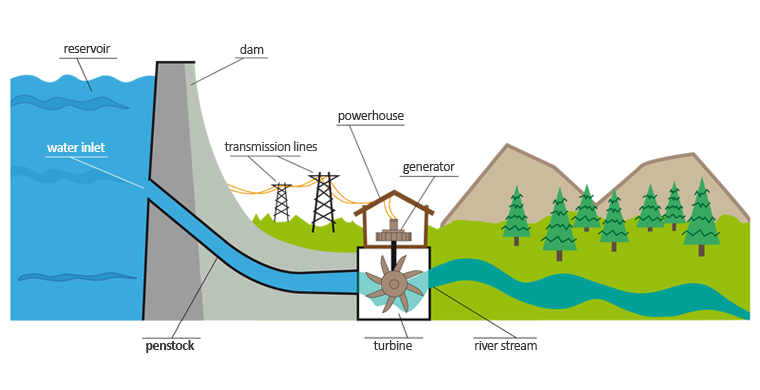
\includegraphics[width=0.6\textwidth]{hydro-with-reservior.png}
\begin{footnotesize}
\vspace{-0.3cm}

Hydro plant with reservoir
%\only<1>{\[\]}

\uncover<2->{Show this information on the second click}
% \vspace{-0.1cm}
\end{footnotesize}

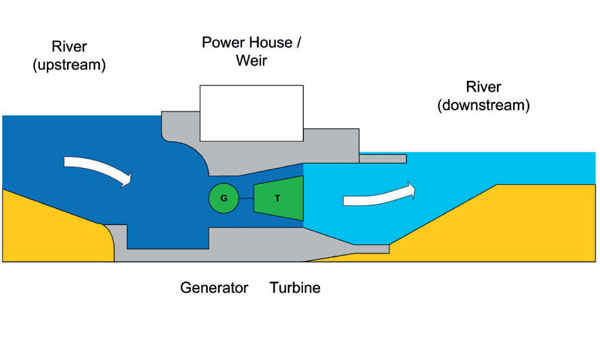
\includegraphics[width=0.5\textwidth]{hydro-without-reservoir}

\begin{footnotesize}
\vspace{-0.3cm}
Hydro plant without reservoir (run-of-river)
%\only<1>{\[\]}
%\only<1-6>{\[{\color{white} y^t_h + s^t_h =  b^{\xi_t}_{t,h} + \sum_{m \in U(h)} (y^t_m + s^t_m)}\]}

\uncover<2->{Also show this information on the second click}
\vspace{-0.1cm}
\end{footnotesize}
\end{center}
\end{column}
\hspace{-1.5cm}
\begin{column}{0.4\textwidth}
%\vspace{0.6cm}
\begin{center}
\begin{footnotesize}
%\vspace{-0.8cm}
\bit
\item<2-> \textbf{This list only shows up on the second click} 
\item[-]<2-> Item 1
\item[-]<2-> Item 2
\eit
\end{footnotesize}
\end{center}
\end{column}
\end{columns}
\end{frame}

\exclude{
\begin{frame}
\frametitle{Multistage stochastic linear programs (MSLPs)}
\vspace{-0.2cm}
\only<1>{
\begin{block}{General MSLP (nested) formulation}
\vspace{-0.45cm}
\begin{tiny}
\begin{align*}
\min_{(x_1, y_1)\in \X_1(x_0)} f_1(x_1, y_1) & + \mathbb{E}_{\xi_2}\Vast[ \min_{(x_2, y_2)\in \X_2(x_1)} f_2(x_2, y_2) + \mathbb{E}_{\xi_3} \vast[\cdots+\mathbb{E}_{\xi_{T}} \Bigg[\min_{(x_T, y_T)\in \X_T(x_{T-1})} f_T(x_T, y_T)
\Bigg]\vast]\Vast]
\end{align*}  
\end{tiny}
\vspace{-0.45cm}
\end{block}
}
\only<2>{
\begin{block}{General MSLP (nested) formulation}
\vspace{-0.45cm}
\begin{tiny}
\begin{align*}
\min_{(x_1, y_1)\in \X_1(x_0)} {\color{blue} f_1(x_1, y_1) } & + \mathbb{E}_{\xi_2}\Vast[ \min_{(x_2, y_2)\in \X_2(x_1)} f_2(x_2, y_2) + \mathbb{E}_{\xi_3} \vast[\cdots+\mathbb{E}_{\xi_{T}} \Bigg[\min_{(x_T, y_T)\in \X_T(x_{T-1})} f_T(x_T, y_T)
\Bigg]\vast]\Vast]
\end{align*}  
\end{tiny}
\vspace{-0.45cm}
\end{block}
}
\only<3>{
\begin{block}{General MSLP (nested) formulation}
\vspace{-0.45cm}
\begin{tiny}
\begin{align*}
\min_{(x_1, y_1)\in \X_1(x_0)}  f_1(x_1, y_1)  & +\alert{\mathbb{E}_{\xi_2}\Vast[ \min_{(x_2, y_2)\in \X_2(x_1)} f_2(x_2, y_2) + \mathbb{E}_{\xi_3} \vast[\cdots+\mathbb{E}_{\xi_{T}} \Bigg[\min_{(x_T, y_T)\in \X_T(x_{T-1})} f_T(x_T, y_T)
\Bigg]\vast]\Vast]}
\end{align*}  
\end{tiny}
\vspace{-0.45cm}
\end{block}
}
\only<4>{
\begin{block}{General MSLP (nested) formulation}
\vspace{-0.45cm}
\begin{tiny}
\begin{align*}
\min_{(x_1, y_1)\in \X_1(x_0)}  f_1(x_1, y_1)  & +\mathbb{E}_{\xi_2}\Vast[ \min_{(x_2, y_2)\in \X_2(x_1)} {\color{blue} f_2(x_2, y_2) } + \mathbb{E}_{\xi_3} \vast[\cdots+\mathbb{E}_{\xi_{T}} \Bigg[\min_{(x_T, y_T)\in \X_T(x_{T-1})} f_T(x_T, y_T)
\Bigg]\vast]\Vast]
\end{align*}  
\end{tiny}
\vspace{-0.45cm}
\end{block}
}

\only<5>{
\begin{block}{General MSLP (nested) formulation}
\vspace{-0.45cm}
\begin{tiny}
\begin{align*}
\min_{(x_1, y_1)\in \X_1(x_0)}  f_1(x_1, y_1)  & +\mathbb{E}_{\xi_2}\Vast[ \min_{(x_2, y_2)\in \X_2(x_1)} f_2(x_2, y_2) + \alert{\mathbb{E}_{\xi_3} \vast[\cdots+\mathbb{E}_{\xi_{T}} \Bigg[\min_{(x_T, y_T)\in \X_T(x_{T-1})} f_T(x_T, y_T)
\Bigg]\vast]}\Vast]
\end{align*}  
\end{tiny}
\vspace{-0.45cm}
\end{block}
}

\only<6->{
\begin{block}{General MSLP (nested) formulation}
\vspace{-0.45cm}
\begin{tiny}
\begin{align*}
\min_{({\color{blue} x_1}, \alert{y_1})\in \X_1(x_0)}  f_1({\color{blue} x_1}, \alert{y_1})  & +\mathbb{E}_{\xi_2}\Vast[ \min_{({\color{blue} x_2}, \alert{y_2})\in \X_2(x_1)} f_2({\color{blue} x_2}, \alert{y_2}) + \mathbb{E}_{\xi_3} \vast[\cdots+\mathbb{E}_{\xi_{T}} \Bigg[\min_{({\color{blue} x_T}, \alert{y_T})\in \X_T(x_{T-1})} f_T({\color{blue} x_T}, \alert{y_T})
\Bigg]\vast] \Vast]
\end{align*}  
\end{tiny}
\vspace{-0.45cm}
\end{block}
}
\MSS

\uncover<6->{
\begin{footnotesize}
\bit
\item ${\color{blue} x_t}$: state variable, $\alert{y_t}$: (local) control variable 
\item $\X_t(x_{t-1}) := \{({\color{blue} x_t}, \alert{y_t}) \mid A^{\xi_t}_t x_{t-1} + B^{\xi_t}_t{\color{blue} x_t} + C^{\xi_t}_t\alert{y_t} = b^{\xi_t}_t\}$ 
\item $\xi_t$: a random vector with known probability distribution (uncertainty)
%\item<7-> For each stage $t$, there exists a set of $N_t$ {\color{blue} realizations} for $\xi_t$ that are independent of decisions made
\eit
\end{footnotesize}
\begin{center}
\vspace{-0.15cm}
\includegraphics[width=0.8\textwidth]{decision_structure.png}
\end{center}
}
\end{frame}
}
\begin{frame}
\frametitle{Content Slide}
\uncover<1->{
\begin{footnotesize}
\begin{block}{A Multistage Stochastic Formulation}
\vspace{-0.2cm}
\begin{tiny}
\begin{align*}
\min_{({\color{blue} x_1}, \alert{y_1})\in \X_1(x_0)}  f_1({\color{blue} x_1}, \alert{y_1})  & +\mathbb{E}_{\xi_2}\Vast[ \min_{({\color{blue} x_2}, \alert{y_2})\in \X_2(x_1)} f_2({\color{blue} x_2}, \alert{y_2}) + \mathbb{E}_{\xi_3} \vast[\cdots+\mathbb{E}_{\xi_{T}} \Bigg[\min_{({\color{blue} x_T}, \alert{y_T})\in \X_T(x_{T-1})} f_T({\color{blue} x_T}, \alert{y_T})
\Bigg]\vast] \Vast]
\end{align*}  
\end{tiny}
\vspace{-0.2cm}
\end{block}
\bit
\item Some variable descriptions
\eit
\end{footnotesize}
}
\uncover<2->{
\MSS
\begin{footnotesize}
\begin{block}{A Dynamic Programming Formulation}
\begin{equation*}
Q_t({\color{blue} x_{t-1}},\xi_{t}):= \left\{
\begin{array}{llll}
\displaystyle \underset{{\color{blue} x_t},\alert{y_t}}{\min} &  f_t({\color{blue} x_t},\alert{y_t}) + \mathcal{Q}_{t+1}({\color{blue}x_t})\\
\mbox{s.t.} &  B_t{\color{blue}x_t} + C_t\alert{y_t} = b^{\xi_t}_t - A_t{\color{blue}x_{t-1}}
\end{array}
\right.
\forall \; t = 1, 2, \dots, T
\end{equation*}
\end{block}
\bit
\item Additional details
\eit
\end{footnotesize}
}
\end{frame}

\begin{frame}
\frametitle{Create ``animation'' for slides}
\framesubtitle{Some additional texts as frame subtitle}
\begin{scriptsize}
\begin{columns}
\begin{column}{0.5\textwidth}

\underline{\textbf{Procedure 1}}
\bem
\item Step 1: These texts are the same in both slides
\item Step 2: But the bottom-right image changes
\eem
\end{column}
\begin{column}{0.5\textwidth}
    \underline{\textbf{Procedure 2}}
    \bem
        \item Step 1
        \item Step 2
    \eem
\end{column}
\end{columns}
\end{scriptsize}
\MSS 
\vspace{-0.45cm}
\begin{columns}
\begin{column}{0.5\textwidth}
\begin{center}
    \begin{figure}
        \centering
        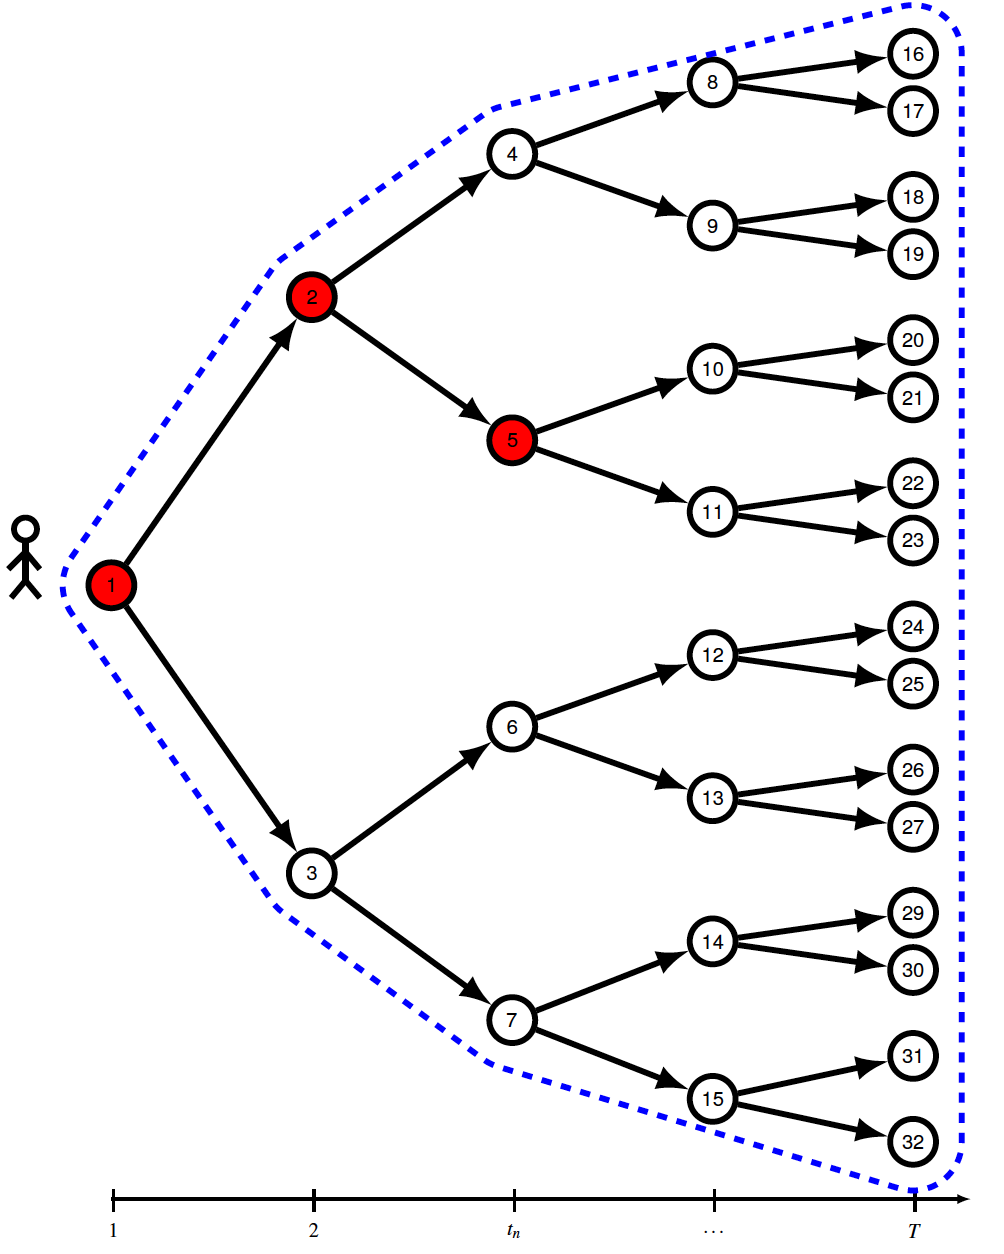
\includegraphics[scale=0.2]{offline.png}
    \end{figure}
\end{center}
\end{column}
\begin{column}{0.5\textwidth}
\begin{center}
    \begin{figure}
        \centering
        \only<1>{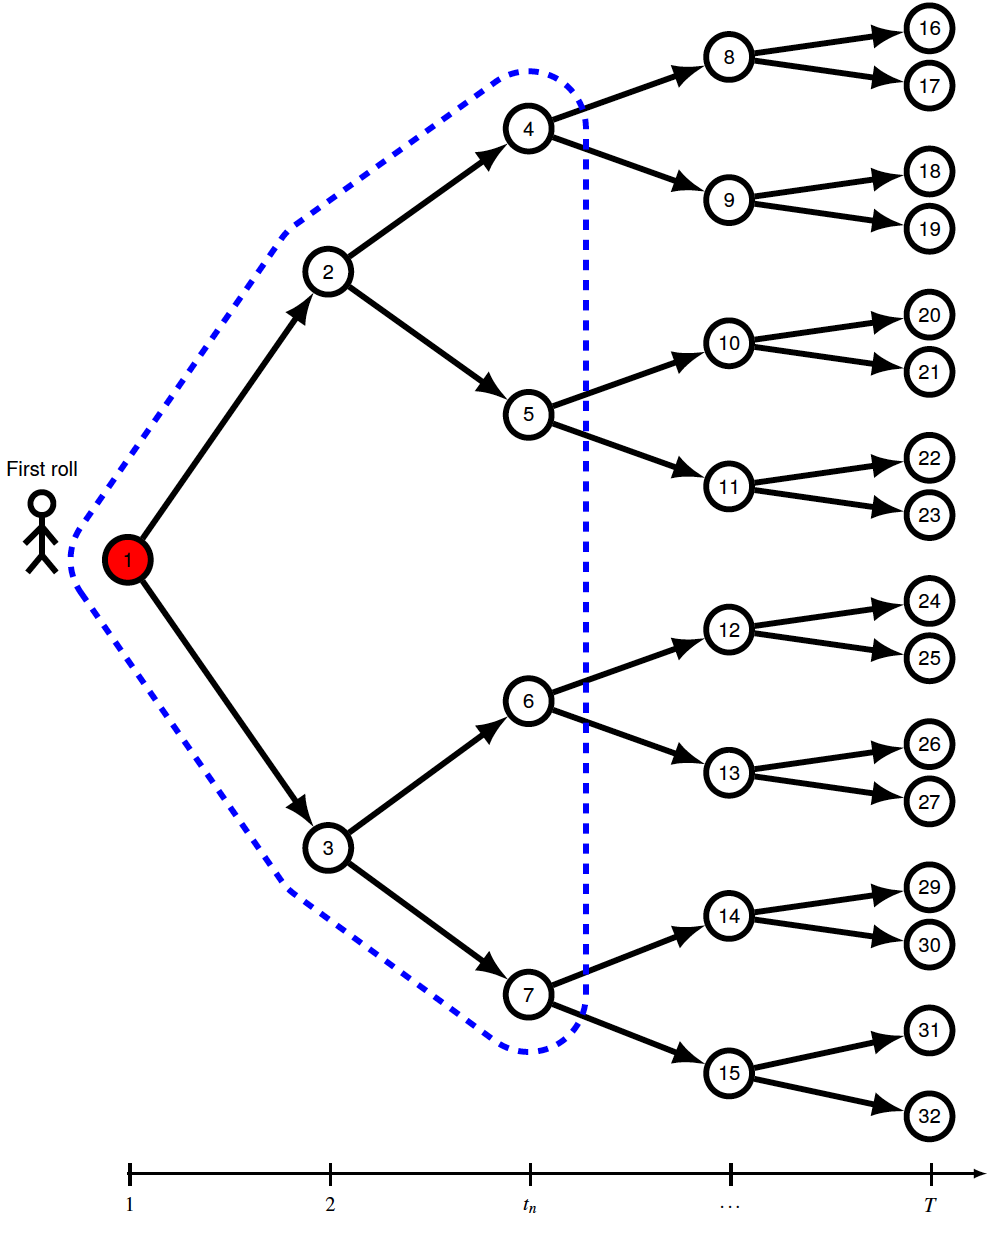
\includegraphics[scale=0.2]{roll1.png}}
        \only<2>{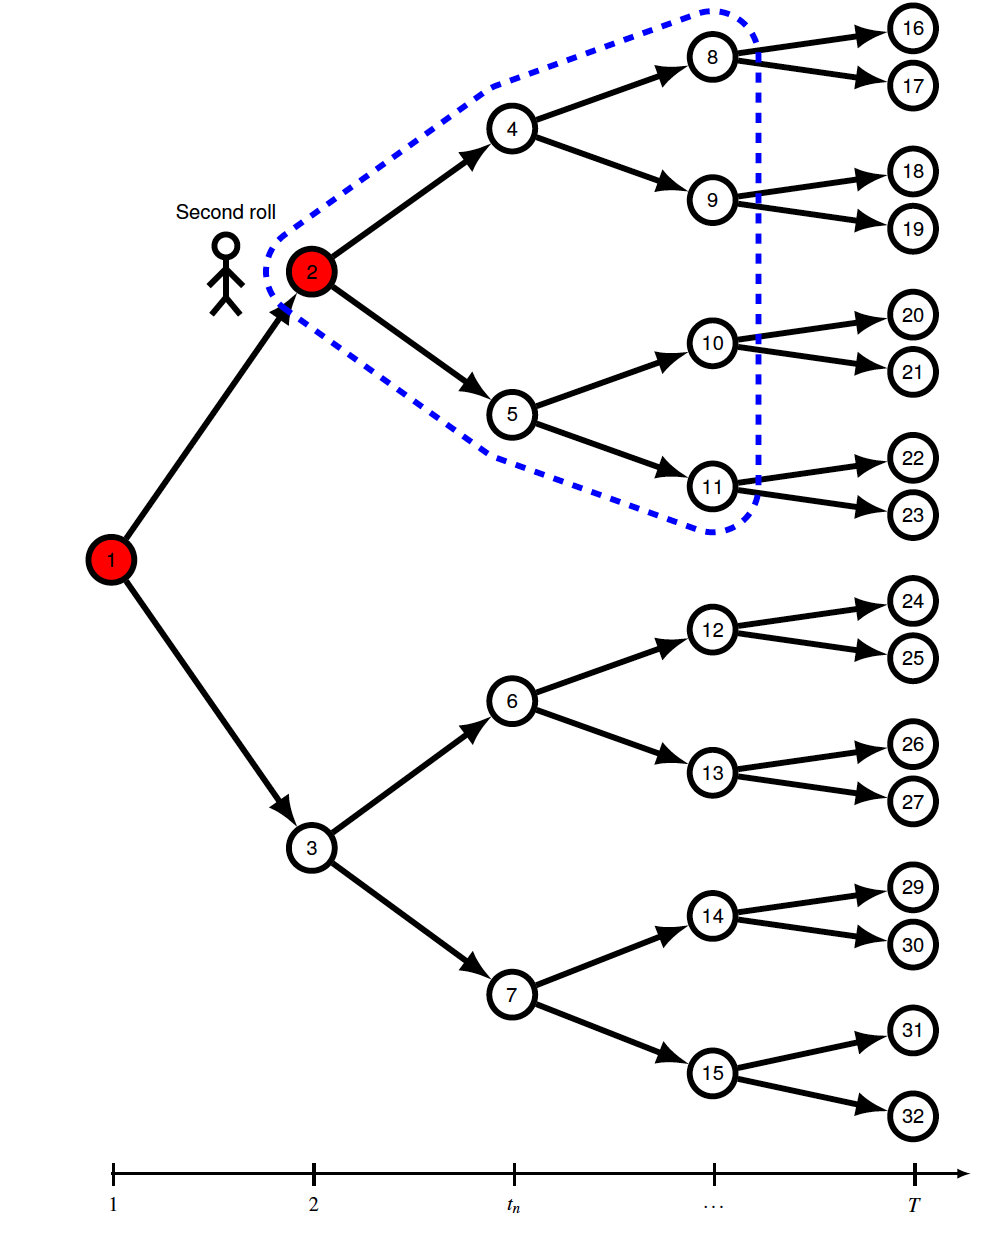
\includegraphics[scale=0.2]{roll2.png}}
    \end{figure}
    \pause 
\end{center}
\end{column}
\end{columns}
\end{frame}

\begin{frame}
\frametitle{A large table for numerical results}

\begin{tiny}
\begin{table}[]
\begin{tabular}{|c|c|c|c|c|c|c|c|c|}
\hline
\multicolumn{3}{|c|}{Instances}                  & \multicolumn{4}{c|}{Optimality Gap}               & \multicolumn{2}{c|}{Training-time (seconds)} \\ \hline
$a$                & $b$              & $c$ & Col A & Col B & Col C & Col D & Col E          & Col F          \\ \hline 
\multirow{8}{*}{1a} & \multirow{4}{*}{2a} & 3   &    &  & & & &   \\
                      & & 4  &   &  & & & &   \\
                      & & 5  &   &  & & & &   \\
                      & & 6  &   &  & & & 1000000&   \\ \cline{2-9} 
                      & \multirow{4}{*}{2b} & 7   & &   &   &  & &    \\
                      & &  8 &   &  & & & &   \\
                      & &  9 &   &  & & & &   \\
                      & &  10 &   &  & & & &   \\ \hline \hline
\multirow{8}{*}{1b} & \multirow{4}{*}{3a} & 11  & & & && &   \\
                        & & 12  &   &  & & & &   \\
                         & &13   &   &  & & & &   \\
                      & &14   &   &  & & & &   \\ \cline{2-9} 
                      & \multirow{4}{*}{3b} &15   &   &  & & & &   \\
                      & & 16  &   &  & & & &   \\
                      & & 17  &   &  & & & &   \\
                      & & 18  &   &  & & & &   \\ \hline
\end{tabular}
\end{table}
\end{tiny}    
\end{frame}

\end{document}
